%% SECTION: GLACIATIONS DURANT LA PERIODE QUATERNAIRE

\paragraph{} La période qui nous intéresse commence il y a 2.6\,MA\footnote{Nous utilisons l'abbréviation MA(kA) pour désigner un million(millier) d'années.} jusqu'à nos jours. Elle est appelée période \emph{quaternaire} et est marquée par la présence d'une calotte glaciaire au pôle nord de la Terre qui a évolué en taille suivant une succession de glaciations importantes, interrompues par de courtes périodes de dégel \cite{wiki_quaternary} \cite{wiki_quaternary_glaciation}. La dernière glaciation a pris fin il y a environ 20000\,ans
\footnote{Il est discutable de séparer la période quaternaire en cette date, car la dernière glaciation est encore très récente. Nous pourrions donc être dans une simple période interglaciaire. L'évolution à long terme du climat est toutefois incertaine, et la tendance semble plutôt être au réchauffement...}
, date qui est parfois utilisée pour séparer la période quaternaire en deux époques: le pléistocène et l'holocène. Le terme pléistocène est donc aussi utilisé pour désigner l'âge des glaciations.



% https://www.giss.nasa.gov/research/briefs/schmidt_01/
\begin{figure}
	\centering
	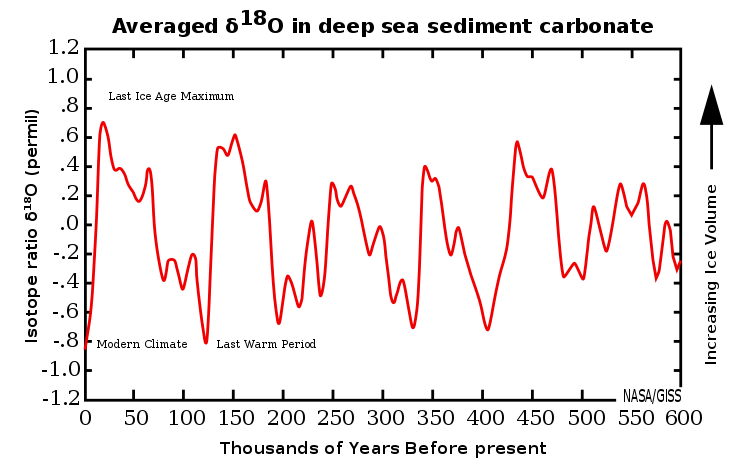
\includegraphics[width=0.9\linewidth]{figures/evol18Osur600kA}
	\caption{Evolution de la présence de $^{18}$O dans les sédiments marins durant les derniers 600\,kA. %La quantité $\delta^{18}$O est un indicateur du volume de glace sur Terre et 
		Son évolution montre une variabilité de 100\,kA dans le climat Terrestre. Image tirée de \cite{giss}.}
	\label{fig:evol18Osur600kA}
\end{figure}

%% https://en.wikipedia.org/wiki/Mid-Pleistocene_Transition
%\begin{figure}
%	\centering
%	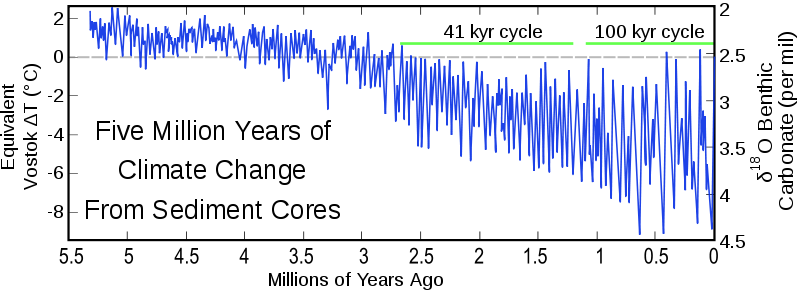
\includegraphics[width=0.9\linewidth]{figures/evol18Osur5MA}
%	\caption{Evolution de la présence de $^{18}$O dans les sédiments marins durant les derniers 5\,MA. Nous observons une variabilité de 41\,kA de 2.6\,MA à 0.9\,MA puis de 100\,kA de 0.9\,MA à nos jours.}
%	\label{fig:evol18Osur5MA}
%\end{figure}
%\todo{fig:cite lisiecki 2005 et wiki mpt}

\begin{figure}
	\centering
	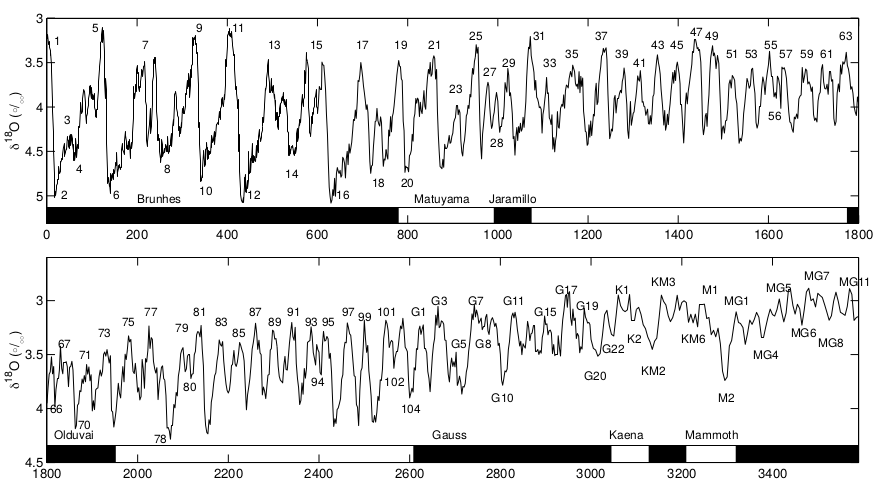
\includegraphics[width=\linewidth]{figures/evol18Osur5MAlisiecki2005}
	\caption{Evolution de la présence de $^{18}$O dans les sédiment marins durant les derniers 5\,MA. Nous observons une variabilité de 41\,kA de 2.6\,MA à 0.9\,MA puis de 100\,kA de 0.9\,MA à nos jours. Image tirée de \cite{lisiecki2005}.}
	\label{fig:evol18Osur5MAlisiecki2005}
\end{figure}



\paragraph{} Les climats passés sont connus à partir de forages, dans de la glace ou des sédiments marins. Plusieurs techniques existent se basant sur la mesure de quantités nous révélant une information sur l'état de la Terre dans le passé. Ces indicateurs peuvent être directs, comme la mesure de la concentration de CO$_2$ dans les carottes de glace, ou indirecte comme la mesure d'abondance relative d'isotopes. La technique la plus fréquente que nous avons rencontré dans ce travail se base sur l'abondance relative des isotopes $^{16}$O et $^{18}$O de l'oxygène dans des sédiments marins de différents types. L'indicateur est défini à partir des mesures d'isotopes selon la formule suivante (voir \cite{wiki_d18O}) 

\begin{equation}\label{d18O}
	\delta^{18}\text{O} = 
	\frac
	{\left(\frac{^{18}\text{O}}{^{16}\text{O}}\right)_{\text{sample}}}
	{\left(\frac{^{18}\text{O}}{^{16}\text{O}}\right)_{\text{standard}}}
	-1 
\end{equation}
et est utilisé pour reconstruire la température de l'environnement dans lequel l'échan- tillon s'est formé ainsi que le volume de glace présent sur les calottes durant les glaciations.

\paragraph{} La figure \ref{fig:evol18Osur600kA} nous renseigne sur l'évolution du climat terrestre durant les derniers 600\,kA \cite{schmidt1999}. Ces données montrent la variation quasi-périodique de la taille des calottes de glace, sur un cycle d'environ 100\,kA. L'évolution sur un temps plus long est donnée sur la figure \ref{fig:evol18Osur5MAlisiecki2005}, basée sur une reconstruction venant de plusieurs sites de forage \cite{lisiecki2005}. Sur cette image, nous pouvons voir une transition dans la périodicité des changement climatique \cite{wiki_mid_pleistocene_transition} \cite{huggett} . Elle se produit il y a environ 900\,kA, au milieu du pléistocène. Les cycles passent d'environ 40\,kA à 100\,kA et augmentent en amplitude. 
